\section{Forudsigelse af indlæggelsesvarigheden}
Ved ortopædkirurgiske operationer er der flere parametre, der kan have indflydelse på indlæggelsesvarigheden. Dette kan eksempelvis være demografiske parametre såsom alder samt køn og kliniske parametre som blodprøver, blodtab og operationstype. Da der kan opstå komplikationer under en operationen, som kan have indflydelse på indlæggelsesvarigheden opdeles parametrene præ- og postoperativt.


\subsection{Præoperativt}
På ortopædkirurgisk afdeling estimeres indlæggelsesvarigheden ikke på nuværende tidspunkt, dog vurderes indlæggelsesforløbet ud fra personalets erfaringer. Ud fra informationspjecer fra ortopædkirurgisk afdeling på Aalborg Universitetshospital informeres om, hvilke faktorer der kan være under en operation. Disse kan angiveligt forlænge indlæggelsesvarigheden. 


\subsubsection{Livsstilsfaktorer}
Livsstilsfaktorer tyder på at have betydning for komplikationer under en operation. Lavt præoperativt funktionsniveau og muskeltab er ofte aldersbetinget, hvilket kan medføre komplikationer og lang indlæggelsesvarighed. Hvorimod patienter med højt funktionsniveau ofte har kortere indlæggelsesvarighed.\cite{Kehlet2001, Janssen2002} Af \figref{alderogindlaeggelse} fremgår patientens alder samt indlæggelsesvarighed i perioden 1. august til den 31. oktober år 2014.


\begin{figure}[H]
	%\flushleft 
	\centering
	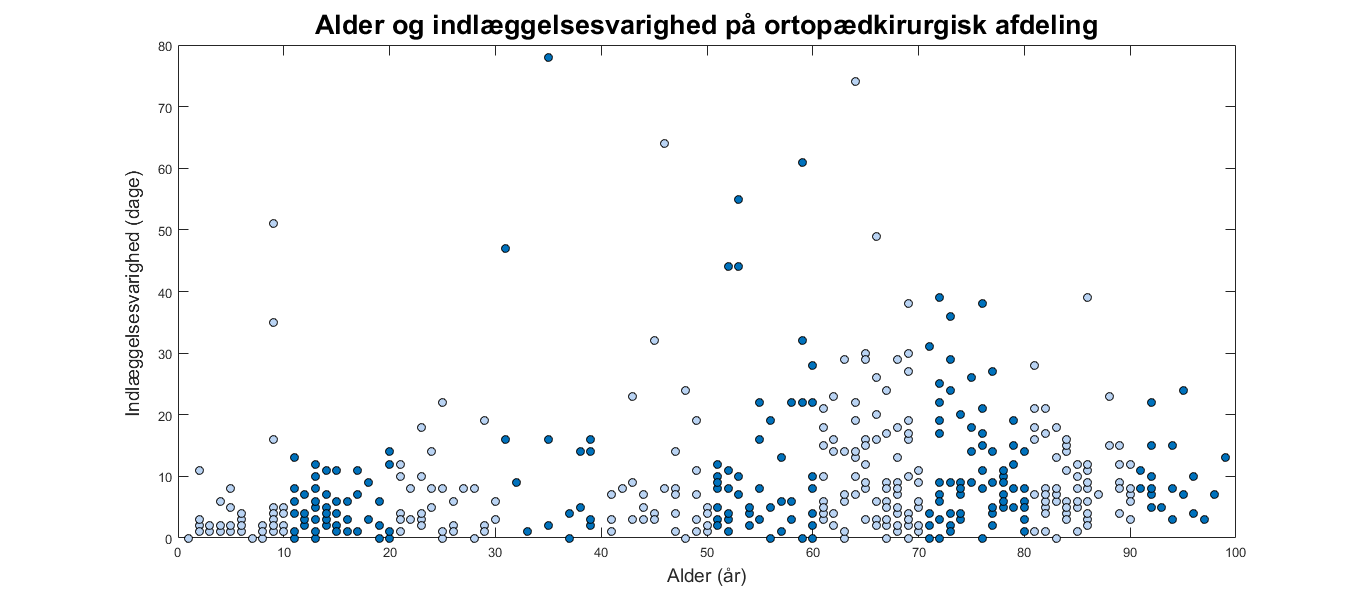
\includegraphics[scale=0.45]{figures/alderogindlaeg}
	%\flushleft
	\caption{\textit{Alder og indlæggelsesvarigheden for patienter på ortopædkirurgisk afdeling. Dette er over en periode på 3 måneder fra den 1. august til den 31. oktober år 2014.}}
	\label{alderogindlaeggelse}
\end{figure}


\noindent
På \figref{alderogindlaeggelse} fremgår det, at der er en bred aldersfordeling på ortopædkirurgisk afdeling. Derudover ses det, at indlæggelsesvarigheden for ældre patienter er mere varierende end yngre patienter, hvoraf denne spredning stiger med alderen. Det fremgår ligeledes, at de ældre patienter indlægges i længere tid end yngre patienter. Patienter under $30$ år er i gennemsnit indlagt 5 dage, hvor patienter over $30$ år i gennemsnit er indlagt 10.9 dage. Det er uvist om dette skyldes lavere funktionsniveau eller om der er andre faktorer der spiller ind, eksempelvis operationstype, som ældre hyppigere får foretaget, hvilket kan medvirke til den længere indlæggelsesvarighed.


Udover alder kan vægt ligeledes have en indflydelse på operationer foretaget på ortopædkirurgisk afdeling, da overvægt giver større risiko for blodpropper\cite{Ermonds2004}. Ved overvægt anbefales det derved at tabe sig før en eventuel operation. Foruden mindsket risiko ved opståen af komplikationer, kan smerter ligeledes reduceres ved vægttab.\cite{Nordjylland2014} På \figref{BMIogindlaeggelse} fremgår body mass index (BMI) samt indlæggelsesvarigheden i samme periode som \figref{alderogindlaeggelse}.

\begin{figure}[H]
	%\flushleft 
	\centering
	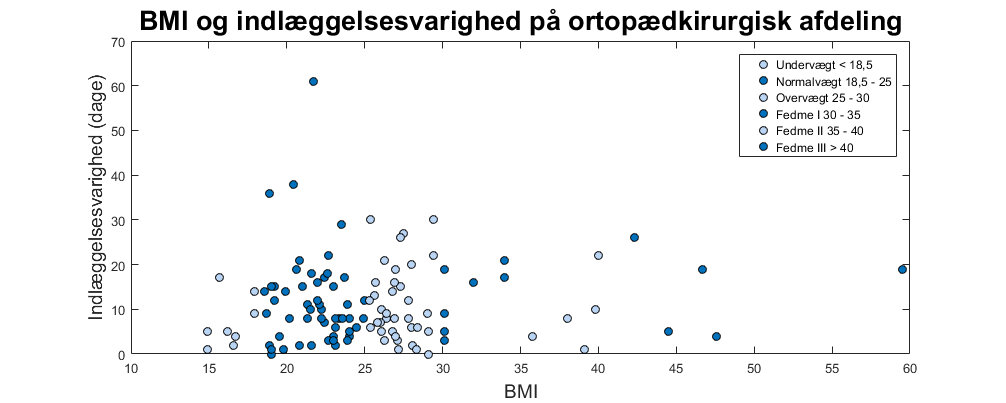
\includegraphics[scale=0.6]{figures/BMIogindlaeg}
	%\flushleft
	\caption{\textit{BMI og indlæggelsesvarigheden for patienter på ortopædkirurgisk afdeling. BMI er opdelt i 6 kategorier: Undervægtig, normalvægtig, overvægt fedme I, fedme II og fedme III. Dette er over en periode på 3 måneder fra den 1. august til den 31. oktober år 2014.}}
	\label{BMIogindlaeggelse}
\end{figure}


\noindent
Af \figref{BMIogindlaeggelse} fremgår det, at størstedelen af patienterne på ortopædkirurgisk afdeling befinder sig inden for vægtklassen, normal og overvægt. Indlæggelsesvarigheden er ligeledes mere varierende i disse klasser, hvor patienterne her er indlagt fra 0 til 61 dage. Indlæggelsesvarigheden er for patienter i normalvægt og overvægt klassen i gennemsnit 11.3, mens det for fedmeklasse I, II, III i gennemsnitlig 11.7 dage. Et højere BMI typer derfor ikke på, at have en betydning for en længere indlæggelsesvarighed. 


Andre livsstilsfaktorer såsom rygning og alkohol kan have betydning for komplikationer under operationer. Rygning kan være medvirkende til at knogler og sår heler langsommere. Ved operationer, hvor der skal transplanteres knoglevæv, f.eks. rygoperationer, afhænger operationens resultat af, at knoglevævet heler rigtigt. Definitionen af en ikke ryger er en person, der har været røgfri i op til 6 måneder, det anbefales derfor at stoppe med at ryge 6 måneder før den planlagte operation.\cite{Nordjylland2014} Fordelingen af ryger, tidligere ryger samt ikke ryger og, hvilken betydning dette har for indlæggelsesvarigheden fremgår af \figref{rygningogindlaeggelse}.


\begin{figure}[H]
	%\flushleft 
	\centering
	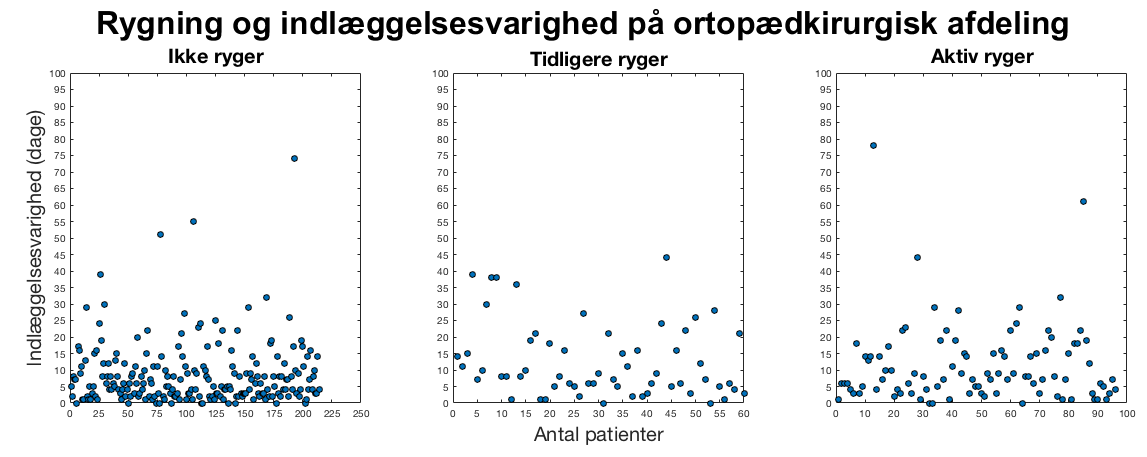
\includegraphics[scale=0.55]{figures/rygerogindlaeg}
	%\flushleft
	\caption{\textit{Rygning og indlæggelsesvarigheden for patienter på ortopædkirurgisk afdeling. Rygning er opdelt efter ikke ryger, eks-ryger og aktiv ryger. Eks-ryger defineres som røgfri i et halvt år. Dette er over en 3 måneders periode fra den 1. august til den 31. oktober år 2014.}}
	\label{rygningogindlaeggelse}
\end{figure}


\noindent
Det ses af \figref{rygningogindlaeggelse}, at størstedelen af ortopædkirurgisk afdeling ikke ryger. Derudover fremgår det, at variationen i indlæggelsesvarigheden er større for eks-rygere og rygere end for aktive rygere. Den gennemsnitlige indlæggelsesvarighed for ikke ryger er 8.4 dage, hvor den for eks-ryger og aktiv er henholdsvis 12.8 og 11 dage. Det tyder derfor på, at rygning har en betydning for indlæggelsesvarigheden.

Som tidligere nævnt kan alkohol ligeledes medføre øget risiko for komplikationer under operationer. Herunder kan der opstå øget blødning under operationer samt infektioner i såret.\cite{Nordjylland2014} Sammenhængen mellem alkohol og indlæggelsesvarigheden er illustreret på  \figref{alkohologindlaeggelse}. 


\begin{figure}[H]
	%\flushleft 
	\centering
	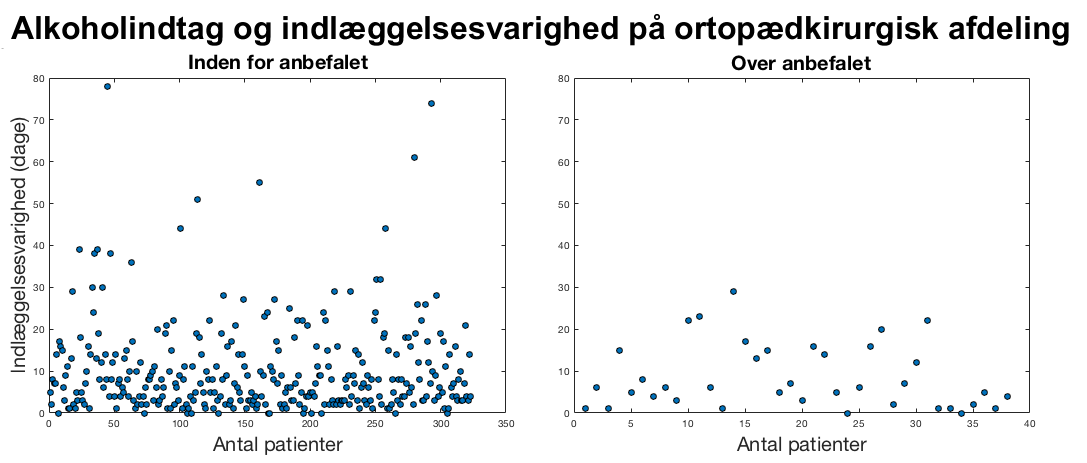
\includegraphics[scale=0.55]{figures/alkohologindlaeg}
	%\flushleft
	\caption{\textit{Alkohol og indlæggelsesvarigheden for patienter på ortopædkirurgisk afdeling. Alkohol er opdelt i inden for anbefalet og over anbefalet. Dette er over en periode på 3 måneder fra den 1. august til den 31. oktober år 2014. }}
	\label{alkohologindlaeggelse}
\end{figure}


\noindent
Det ses af \figref{alkohologindlaeggelse}, at størstedelen af patienter på ortopædkirurgisk afdeling befinder sig inden for anbefalingen af alkoholindtag. Den gennemsnitlige indlæggelsestid for patienter der holder sig inden for det anbefalede er 10 dage, mens den for patienter der drikker over anbefalet er indlagt 8.4 dage. Det tyder derfor på, at patienter der drikker inden for anbefalet er indlagt i længere tid. 

Det tyder på, at livsstilsfaktorer som komorbiditeter har betydning for indlæggelsesvarigheden. Patienter med komorbiditeter f.eks. dårligt blodomløb og diabetes kræver ofte særlig behandling. Diabetes har blandt andet betydning ift. sårheling \ref{interview}. Af figur \figref{diabetesogindlaeggelse} fremgår diabetes og indlæggelsesvarigheden. 

%\begin{figure}[H]
%	%\flushleft 
%	\centering
%	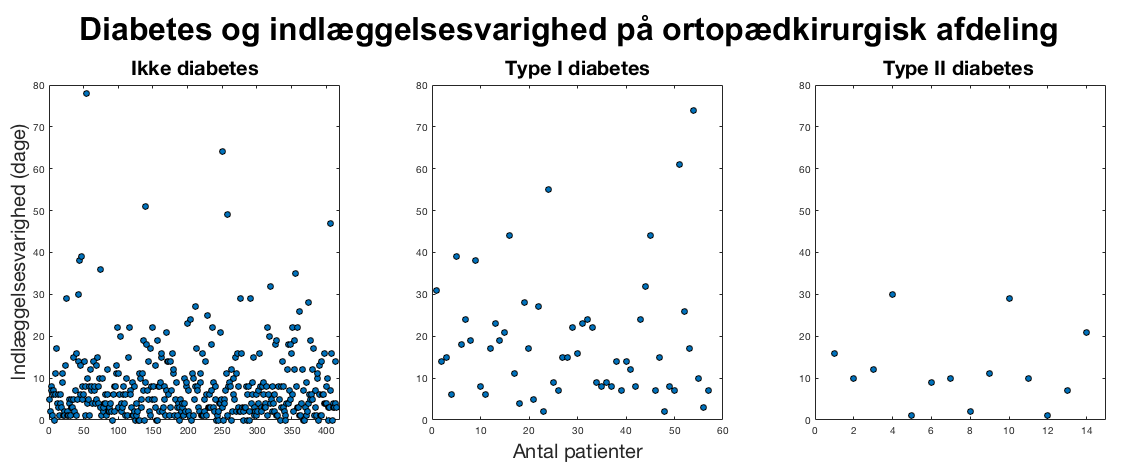
\includegraphics[scale=0.55]{figures/diabetesogindlaeg}
%	%\flushleft
%	\caption{\textit{Alkohol og indlæggelsesvarigheden for patienter på ortopædkirurgisk afdeling. Alkohol er opdelt i inden for anbefalet og over anbefalet. Dette er over en periode på 3 måneder fra den 1. august til den 31. oktober år 2014. }}
%	\label{diabetesogindlaeggelse}
%\end{figure}

\noindent
På \figref{diabetesogindlaeggelse}

**** SKAL SKRIVES HER ***


\subsubsection{Indgreb}
Som beskrevet i \ref{kap_OA} udføres flere operationstyper med forskellig varighed på ortopædkirurgisk afdeling, hvorfor det forventes at indlæggelsesvarigheden ligeledes er varierende. 


\begin{figure}[H]
	%\flushleft 
	\centering
	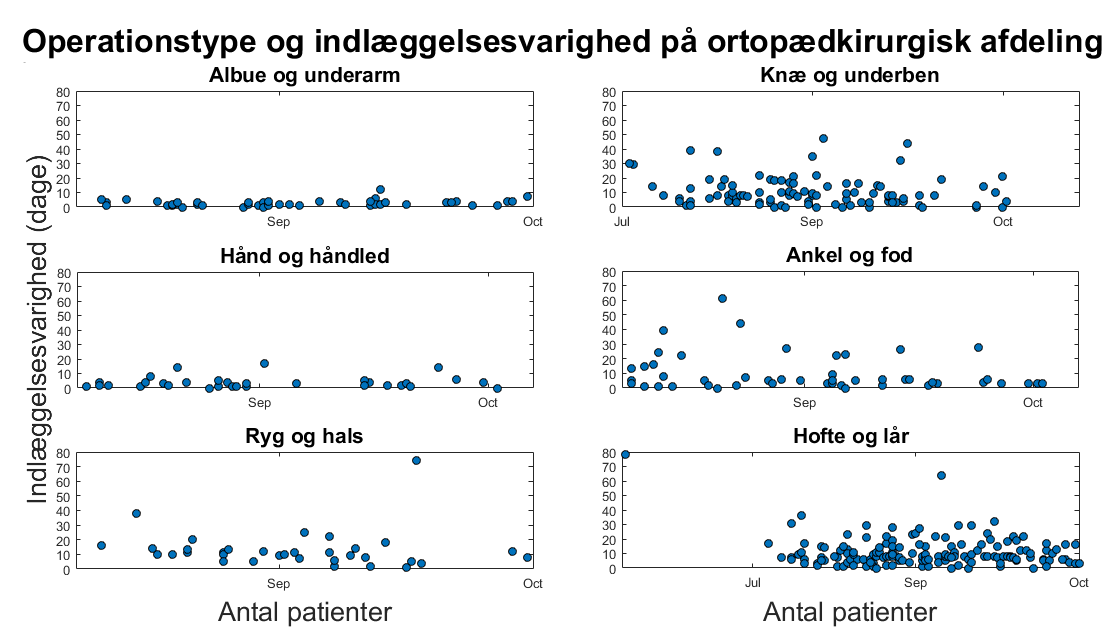
\includegraphics[scale=0.5]{figures/operaogindlaeg}
	%\flushleft
	\caption{\textit{Operationstyper og indlæggelsesvarigheden for patienter på ortopædkirurgisk afdeling. Operationstyper er opdelt efter albue og underarm, hånd og håndled, ryg og hals, knæ og underben, ankel og fod samt hofte og lår. Dette er over en periode på 3 måneder fra den 1. august til den 31. oktober år 2014.}}
	\label{opvsindlaegtid}
\end{figure}


\noindent
På \figref{opvsindlaegtid} fremgår det, at indlæggelsesvarigheden er varierende for typen af operation, hvoraf den gemmesnitlige indlæggesesvarighed er fra 2.7 dage op til 12.5 dage.  Den gennemsnitlige  indlæggelsesvarighed er for ryg og hals, hofte og lår, knæ og underben samt ankel og fod, henholdsvis 12.5, 10.8, 10.2 og 10.1 dage. Modsat er den gennemsnitlige indlæggelsesvarighed for hånd og håndled samt albue og underarm 3.8 og 2.7 dage. Hertil tyder det på, at indlæggelsesvarigheden er længere for operationer foretaget på underekstremiteter sammenlignet med overekstremiteter. Derudover ses det, at de fleste operationer der foretages på ortopædkirurgisk afdeling er en hofte og lår eller knæ og underben operation. 



\subsubsection{Tilgængelige kirurger}
Det kan i nogle tilfælde være nødvendigt at udsætte elektive patienters operationer, hvis et akut tilfælde opstår, hvorved kirurgen skal være til stede. Derved kan patienter indlæggelsesvarighed forlænges. Ved udsættelse af elektive patienter vil denne ofte få en ny tid hurtigst muligt. Den nye tid vil typisk være først på dagen, således risikoen for endnu en udsættelse mindskes.